\documentclass[letterpaper,10pt]{article}
\usepackage[top=2cm, bottom=1.5cm, left=1cm, right=1cm]{geometry}
\usepackage{amsmath, amssymb, amsthm,graphicx}
\usepackage{fancyhdr}
\pagestyle{fancy}

\lhead{\today}
\chead{MV Stats Assignment 2}
\rhead{Justin Hood}

\newcommand{\Z}{\mathbb{Z}}
\newcommand{\Q}{\mathbb{Q}}
\newcommand{\R}{\mathbb{R}}
\newcommand{\C}{\mathbb{C}}
\newtheorem{lem}{Lemma}

\begin{document}
\begin{description}
\item[Problem 2.1]\hfill\\
Let,
\[x=\begin{bmatrix}
5 & 1 & 3
\end{bmatrix},\ y=\begin{bmatrix}
-1 & 3 & 1
\end{bmatrix} \]
Plotting, we find,
\begin{center}
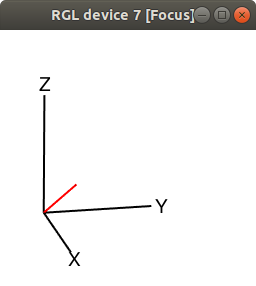
\includegraphics[scale=0.5]{1x.png}
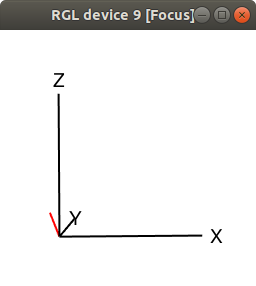
\includegraphics[scale=0.5]{1y.png}
\end{center}
Using $R$, we compute that,
\begin{align*}
|x|&=\sqrt{5^2+1^2+3^2}\\
&=\sqrt{35}\approx 5.91608\\
|y|&=\sqrt{-1^2+3^2+1^2}\\
&=\sqrt{11}\approx 3.3166
\end{align*}
The angle is then,
\[\cos(\theta)=\frac{x'y}{|x||y|}=\frac{1}{\sqrt{35}\sqrt{11}}\approx 0.050964\Rightarrow \theta=1.51981rad=87.07867\deg\]
Finally, the projection of $x$ onto $y$ is computed as,
\[proj=\frac{x'y}{L_y^2}y=\begin{bmatrix}
\frac{-1}{11}\\
\frac{2}{11}\\
\frac{1}{11}
\end{bmatrix} \]
Plotting the adjusted vectors in red with the original blue,
\begin{center}
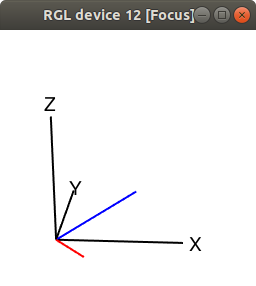
\includegraphics[scale=0.5]{1n.png}
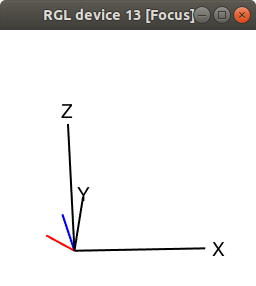
\includegraphics[scale=0.5]{1m.png}
\end{center}
We see that these are inverses of eachother.
\item[Problem 2.5]\hfill\\
We consider,
\[\textbf{Q}=\begin{bmatrix}
\frac{5}{13} & \frac{12}{13}\\
\frac{-12}{13} & \frac{5}{13}
\end{bmatrix} \]
If this matrix is Orthogonal, then $\textbf{Q'Q}=I$. Using, $R$, we compute,
\[\textbf{Q'Q}=\begin{bmatrix}
1 & 0\\
0 & 1
\end{bmatrix}\]
As desired.
\item[Problem 2.6]\hfill\\
We shall let,
\[A=\begin{bmatrix}
9 & -2\\ -2 & 6
\end{bmatrix}\]
We see that $A$ is symmetric, as $A=A'$. Using $R$, we compute the eigenvalues to be,
\[\Lambda=\begin{bmatrix}
10\\5
\end{bmatrix}\]
Because these eigenvalues are greater than zero, we see that the matrix is indeed positive definite.
\item[Problem 2.8]\hfill\\
Consider the matrix
\[A=\begin{bmatrix}
1 & 2\\ 2 & -2
\end{bmatrix} \]
We compute the eigenvalues as follows:
\begin{align*}
A-\lambda I &= \begin{bmatrix}
1-\lambda & 2\\ 2 & -2-\lambda
\end{bmatrix}
0 &= (1-\lambda)(-2-\lambda)-4
\end{align*}
Solving, we find that $\Lambda=[2,-3]$
Plugging this in, we compute the eigenvectors as,
\begin{align*}
A-2I &= \begin{bmatrix}
-1 & 2 \\ 2 & -4
\end{bmatrix}
&=\begin{bmatrix}
1 & -2\\ 0 & 0
\end{bmatrix}
\end{align*}
Thus, we see that the eigenvector for this value is,
\[e_1=\begin{bmatrix}
2 \\1
\end{bmatrix} \]
Similarly, the vector for the other eigenvalue is computed to be,
\[e_2=\begin{bmatrix}
1 \\ -2
\end{bmatrix}\]
Normalizing, we find that these vectors become,
\[e_1=\begin{bmatrix}
\frac{2}{\sqrt{5}}\\ \frac{1}{\sqrt{5}}
\end{bmatrix},\ e_2=\begin{bmatrix}
\frac{1}{\sqrt{5}}\\\frac{-2}{\sqrt{5}}
\end{bmatrix} \]
Finally, the spectral decomposition of $A$ becomes,
\[A=\lambda_1e_1'e_1+\lambda_2e_2'e_2\]
Which is easily verified in $R$.
\item[Problem 2.9]\hfill\\
Using $A$ as above, we compute $A$ inverse using the equation presented in the text,
\[A^{-1}=\frac{1}{|A|}\begin{bmatrix}
a_{22} & -a_{12}\\ -a_{21} & a_{11}
\end{bmatrix} \]
$A^{-1}$ is then,
\[A^{-1}=\begin{bmatrix}
1/3 & 1/3\\1/3 & -1/6
\end{bmatrix}\]
The eigenvalues and associated eigenvectors are then,
\begin{align*}
\Lambda &= \begin{bmatrix}
1/2 \\ -1/3
\end{bmatrix}\\
e_1 &= \begin{bmatrix}
2/\sqrt{5} \\ 1/\sqrt{5}
\end{bmatrix}\\
e_2 &= \begin{bmatrix}
1/\sqrt{5}\\-2/\sqrt{5}
\end{bmatrix}
\end{align*}
The spectral decomposition is then,
\[A=\lambda_1e_1'e_1+\lambda_2e_2'e_2\]
We see that the eigenvectors are the same as before, and the eigenvalues are merely the inverses of those from before.
\item[Problem 2.15]\hfill\\
Consider the quadratic form,
\[3x_1^2+3x_2^2-2x_1x_2\]
We first convert this to an equation of the form,
\[x'Ax\]
Then,
\[A=\begin{bmatrix}
3 & -1\\-1 & 3
\end{bmatrix}\]
We shall now compute the eigenvalues with $R$,
\[\Lambda=\begin{bmatrix}
4 \\ 2
\end{bmatrix} \]
Since these are both positive values, we see that the quadratic is indeed positive definite.
\item[Problem 2.16]\hfill\\
We consider the arbitrary matrix $A$ with dimension $n\times p$. Then, $A'A$ is a symmetric matrix with dimension $p\times p$. Now, let $y=Ax$ as described. We now compute,
\begin{align*}
y'y &= (Ax)'Ax\\
&= (x'A')Ax
\end{align*}
The equation $y'y$ looks similar to the form of the quadratic $x'Ax$ from the text. If the quadratic is non-negative then we may conclude $A$ is non-negative. Here, ``A" is $A'A$. Now, we note that,
\[y=\begin{bmatrix}
y_1\\y_2\\\vdots\\y_p
\end{bmatrix}\]
A vector of dimension $p$. So,
\[y'y=y_1^2+y_2^2+\ldots y_p^2\]
This function is a sum of squares, and is thus greater than or equal to zero. Now,
\[y'y=x'A'Ax\geq 0 \]
We see that the matrix $A'A$ is non-negative definite as desired.
\item[Problem 2.18]\hfill\\
We consider the points $(x_1,\ x_2)$ defined by the distance to the origin by,
\[c^2=4x_1^2+3x_2^2-2\sqrt{2}x_1x_2\]
We note that the RHS of this equation can be rewritten as,
\[x'Ax=[x_1,\ x_2]\begin{bmatrix}
4 & -\sqrt{2}\\-\sqrt{2} & 3
\end{bmatrix}\begin{bmatrix}
x_1\\x_2
\end{bmatrix} \]
The matrix $A$ then has the eigenvalues $\Lambda=[2,\ 5]$
And normalized eigenvectors,
\[e_1=\begin{bmatrix}
1/\sqrt{3}\\\sqrt{2}/\sqrt{3}
\end{bmatrix},\ e_2=\begin{bmatrix}
\sqrt{2}/\sqrt{3} \\ -1/\sqrt{3}
\end{bmatrix} \]
For $c^2=1$, the major axis has length,
\[\frac{c}{\sqrt{\lambda_1}}=\frac{1}{\sqrt{2}}=0.7071\]
And the minor,
\[\frac{c}{\sqrt{\lambda_2}}=\frac{1}{\sqrt{5}}=0.4472\]
These axes follow the ordained eigenvectors from above.\\
For $c^2=4$, the major axis has length,
\[\frac{c}{\sqrt{\lambda_1}}=\frac{2}{\sqrt{2}}=1.4142\]
And the minor,
\[\frac{c}{\sqrt{\lambda_2}}=\frac{2}{\sqrt{5}}=0.89443\]
Thus, we see that as $c^2$ increases, the lengths of the sides increase as well.
\item[Problem 2.21]\hfill\\
We consider the matrix,
\[A=\begin{bmatrix}
1 & 1\\2 & -2\\2 & 2
\end{bmatrix}\]
Then,
\[A'A=\begin{bmatrix}
9 & 1\\1 & 9
\end{bmatrix}\]
With associated eigen values and vectors,
\[\Lambda=\begin{bmatrix}
10\\8
\end{bmatrix} \]
\[e_1=\begin{bmatrix}
1/\sqrt{2} \\ 1/\sqrt{2}
\end{bmatrix},\ e_2=\begin{bmatrix}
1/\sqrt{2} \\ -1/\sqrt{2}
\end{bmatrix} \]
We now compute the same things, for the value $AA'$.
\[AA'=\begin{bmatrix}
2 & 0 & 4\\
0 & 8 & 0\\
4 & 0 & 8
\end{bmatrix} \]
\[\Lambda=\begin{bmatrix}
10\\8\\0
\end{bmatrix} \]
\[e_1=\begin{bmatrix}
1/\sqrt{5}\\0\\2/\sqrt{5}
\end{bmatrix},\ e_2=\begin{bmatrix}
0\\1\\0
\end{bmatrix},\ e_3=\begin{bmatrix}
2/\sqrt{5}\\0\\-1/\sqrt{5}
\end{bmatrix} \]
The decomposition is then,
\[A=\sqrt{10}\begin{bmatrix}
1/\sqrt{5}\\0\\2/\sqrt{5}
\end{bmatrix}\begin{bmatrix}
1/\sqrt{2} & 1/\sqrt{2}
\end{bmatrix}+\sqrt{8}\begin{bmatrix}
0\\1\\0
\end{bmatrix}\begin{bmatrix}
1/\sqrt{2} & -1/\sqrt{2}
\end{bmatrix}=\begin{bmatrix}
1 & 1\\2 & -2\\2 & 2
\end{bmatrix} \]
As desired.
\item[Problem 2.23]\hfill\\
We consider the covariance matrix defined as,
\[\Sigma=\begin{bmatrix}
\sigma_{11} & \sigma_{12} & \ldots & \sigma_{1p}\\
\sigma_{21} & \sigma_{22} & \ldots & \sigma_{2p}\\
\vdots & \vdots & \ddots & \vdots\\
\sigma_{p1} & \sigma_{p2} & \ldots & \sigma_{pp}
\end{bmatrix} \]
And the standard deviation matrix
\[V^{1/2}=\begin{bmatrix}
\sqrt{\sigma_{11}} & 0 & \ldots & 0\\
0 & \sqrt{\sigma_{22}} & \ldots & 0\\
\vdots & \vdots & \ddots & \vdots\\
0 & 0 & \ldots & \sqrt{\sigma_{pp}}
\end{bmatrix} \]
We now consider,
\[(V^{1/2})^{-1}\Sigma(V^{1/2})^{-1}=\begin{bmatrix}
1/\sqrt{\sigma_{11}} & 0 & \ldots & 0\\
0 & 1/\sqrt{\sigma_{22}} & \ldots & 0\\
\vdots & \vdots & \ddots & \vdots\\
0 & 0 & \ldots & 1/\sqrt{\sigma_{pp}}
\end{bmatrix}\begin{bmatrix}
\sigma_{11} & \sigma_{12} & \ldots & \sigma_{1p}\\
\sigma_{21} & \sigma_{22} & \ldots & \sigma_{2p}\\
\vdots & \vdots & \ddots & \vdots\\
\sigma_{p1} & \sigma_{p2} & \ldots & \sigma_{pp}
\end{bmatrix} \begin{bmatrix}
1/\sqrt{\sigma_{11}} & 0 & \ldots & 0\\
0 & 1/\sqrt{\sigma_{22}} & \ldots & 0\\
\vdots & \vdots & \ddots & \vdots\\
0 & 0 & \ldots & 1/\sqrt{\sigma_{pp}}
\end{bmatrix}\]
Because of the zeros on the nondiagonal entries in the $V$ matrices, this simplifies to,
\[\begin{bmatrix}
\frac{\sigma_{11}}{\sqrt{\sigma_{11}}\sqrt{\sigma_{11}}} & \frac{\sigma_{12}}{\sqrt{\sigma_{11}}\sqrt{\sigma_{22}}} & \ldots & \frac{\sigma_{1p}}{\sqrt{\sigma_{11}}\sqrt{\sigma_{pp}}}\\
\frac{\sigma_{21}}{\sqrt{\sigma_{22}}\sqrt{\sigma_{11}}} & \frac{\sigma_{22}}{\sqrt{\sigma_{22}}\sqrt{\sigma_{22}}} & \ldots & \frac{\sigma_{2p}}{\sqrt{\sigma_{22}}\sqrt{\sigma_{pp}}}\\
\vdots & \vdots & \ddots & \vdots\\
\frac{\sigma_{1p}}{\sqrt{\sigma_{11}}\sqrt{\sigma_{pp}}} & \ldots & \ldots & \frac{\sigma_{pp}}{\sqrt{\sigma_{pp}}\sqrt{\sigma_{pp}}}
\end{bmatrix}=\rho\]
We note that the entries on the diagonal are equal to one, and the remaining entries are the various population correlation values we have previously computed. Now,
\begin{align*}
(V^{1/2})^{-1}\Sigma(V^{1/2})^{-1}&=\rho && \Leftrightarrow\\
V^{1/2}(V^{1/2})^{-1}\Sigma(V^{1/2})^{-1}V^{1/2} &= V^{1/2}\rho V^{1/2} && \Leftrightarrow\\
\Sigma &= V^{1/2}\rho V^{1/2}
\end{align*}
As desired.
\item[Problem 2.25]\hfill\\
Let $X$ have the covariance matrix,
\[\Sigma=\begin{bmatrix}
25 & -2 & 4\\
-3 & 4 & 1\\
4 & 1 & 9
\end{bmatrix} \]
Using the formulas defined in the previous problem, we compute the matrices,
\[V^{1/2}=\begin{bmatrix}
5 & 0 & 0\\
0 & 2 & 0\\
0 & 0 & 3
\end{bmatrix} \]
\[\rho=\begin{bmatrix}
1 & -1/5 & 4/15\\
-1/5 & 1 & 1/6\\
4/15 & 1/6 & 1
\end{bmatrix} \]
Using $R$, we compute,
\[V^{1/2}\rho V^{1/2} = \begin{bmatrix}
25 & -2 & 4\\
-3 & 4 & 1\\
4 & 1 & 9
\end{bmatrix}=\Sigma \]
As desired.
\item[Problem 2.26]\hfill\\
From before,
\[\sigma_{13}=\frac{4}{15}\]
We now consider the correlation between $X_1$ and $1/2X_2+1/2X_3$
\[Cor(X_1,\ 1/2X_2+1/2X_3)=\frac{cov(X_1,\ 1/2X_2+1/2X_3)}{\sqrt{Var(X_1)}\sqrt{Var(1/2X_2+1/2X_3)}}\]
From before, we know that $Var(X_1)=25=\sigma_{11}$.\\
Next,
\[Var(1/2X_2+1/2X_3)=\frac{1}{2^2}\sigma_{22}+\frac{1}{2}\sigma_{33}+2(\frac{1}{2^2}\sigma_{23})=1+\frac{9}{4}+\frac{1}{2}=\frac{15}{4}\]
Finally,
\[cov(X_1,\ 1/2X_2+1/2X_3)=\frac{\sigma_{12}}{2}+\frac{\sigma_{13}}{2}=-1+2=1\]
So,
\[Cor(X_1,\ 1/2X_2+1/2X_3)=\frac{1}{\sqrt{25}\sqrt{15/4}}=0.10328\]
\end{description}
\end{document}
